%! Author = Sujal Singh
%! Date = 5/24/24

% Preamble
%! suppress = FileNotFound
\documentclass[11pt]{ipu-r}

% Packages
\usepackage{amsmath}
\usepackage{lmodern}
\usepackage[margin=2cm]{geometry}
\usepackage{tabularray}

% Document
\begin{document}
    \fancypagestyle{empty}{%
        \fancyhf{}
        \fancyfoot[C]{Page \thepage}
        \renewcommand{\headrulewidth}{0pt}
        \renewcommand{\footrulewidth}{0.4pt}
    }
    \pagestyle{empty}
    \noindent\textbf{
        \begin{center}
            \vspace*{-30pt}%
            \noindent{Guru Gobind Singh Indraprastha University, East Delhi Campus%
            \\[8pt]End Term Practical Examination Solved Paper (IIOT--B1--B, 2024)\\[10pt]}
        \end{center}
        Paper Code: BS110P \hfill Subject: Probability \& Statistics for Engineers Lab
        \\[8pt]
        Time: 1.5 hour \hfill Max Marks: 50?
        \\[8pt]
        Note: All questions are compulsory.\\\hline%
    }
    \\~\\[20pt]%
    %------------------------------------------------------------------------------------------------------------------%
    \firstquestion{Solve the following system of equations:
        \begin{align*}
            x + y + z &= 3\\
            2x - y + 3z &= 4\\
            3x - 2y + z &= 0
        \end{align*}\vspace*{-20pt}}
    \begin{code}
        {Program}{r}
A <- matrix(c(1, 2, 3, 1, -1, -2, 1, 3, 1), ncol=3)
b <- matrix(c(3, 4, 0))
solve(A, b)
    \end{code}
    \begin{code}
        {Output}{text}
          [,1]
[1,] 0.2727273
[2,] 1.1818182
[3,] 1.5454545
    \end{code}
    %------------------------------------------------------------------------------------------------------------------%

    %------------------------------------------------------------------------------------------------------------------%
    \question{Create 30 random numbers from binomial distribution $\mathbf{B(40, 0.25)}$.}
    \begin{code}
        {Program}{r}
rbinom(30, size=40, prob=0.25)
    \end{code}
    \begin{code}
        {Output}{text}
 [1]  9  7  6 10  6  9 10 10 11 13 11  6  7 12 11  6 14 10
[19] 11 11  8 10  5 10  8  7 12  9 12 11
    \end{code}
    %------------------------------------------------------------------------------------------------------------------%

    %------------------------------------------------------------------------------------------------------------------%
    \question{Create two matrices of order $\mathbf{3x4}$. Add and subtract them. Also, find the transpose of both
    matrices.}
    \begin{code}
        {Program}{r}
a <- matrix(1:12, nrow=3)
b <- matrix(1:12, nrow=3, byrow=TRUE)

a + b
a - b

t(a)
t(b)
    \end{code}
    \newpage
    \vspace*{-10pt}
    \begin{code}
        {Output}{text}
     [,1] [,2] [,3] [,4]
[1,]    2    6   10   14
[2,]    7   11   15   19
[3,]   12   16   20   24
     [,1] [,2] [,3] [,4]
[1,]    0    2    4    6
[2,]   -3   -1    1    3
[3,]   -6   -4   -2    0
     [,1] [,2] [,3]
[1,]    1    2    3
[2,]    4    5    6
[3,]    7    8    9
[4,]   10   11   12
     [,1] [,2] [,3]
[1,]    1    5    9
[2,]    2    6   10
[3,]    3    7   11
[4,]    4    8   12
    \end{code}
    %------------------------------------------------------------------------------------------------------------------%

    %------------------------------------------------------------------------------------------------------------------%
    \question{Create a data frame of 5 scholars with their names, marks in project 1, project 2, project 3. Find mean
    and variance of project 2.}
    \begin{code}
        {Program}{r}
dataset <- data.frame(
  "Project1" = c(77, 83, 93, 67, 89),
  "Project2" = c(50, 79, 89, 29, 84),
  "Project3" = c(92, 95, 99, 81, 98),
  row.names = c("Alice", "Bob", "Eve", "John", "Jane")
)

project2_marks <- dataset[,2]
mean(project2_marks)
var(project2_marks)
    \end{code}
    \begin{code}
        {Output}{text}
[1] 66.2
[1] 661.7
    \end{code}
    %------------------------------------------------------------------------------------------------------------------%

    %------------------------------------------------------------------------------------------------------------------%
    \question{Draw histogram of:\\[10pt]
        \begin{center}
            \begin{tblr}{colsep=10pt,rowsep=10pt,hlines,vlines}
                CI           & 0--25 & 25--500 & 50--75 & 75--100 & 100--125 \\
                $\mathbf{f}$ & $5$   & $8$     & $13$   & $11$    & $3$
            \end{tblr}
        \end{center}}
    \newpage
    \begin{code}
        {Program}{r}
barplot(
  height=c(5, 8, 13, 11, 3),
  names.arg = c("0-25", "25-50", "50-75", "75-100", "100-125"),
  xlab="CI",
  ylab="f"
)
    \end{code}
    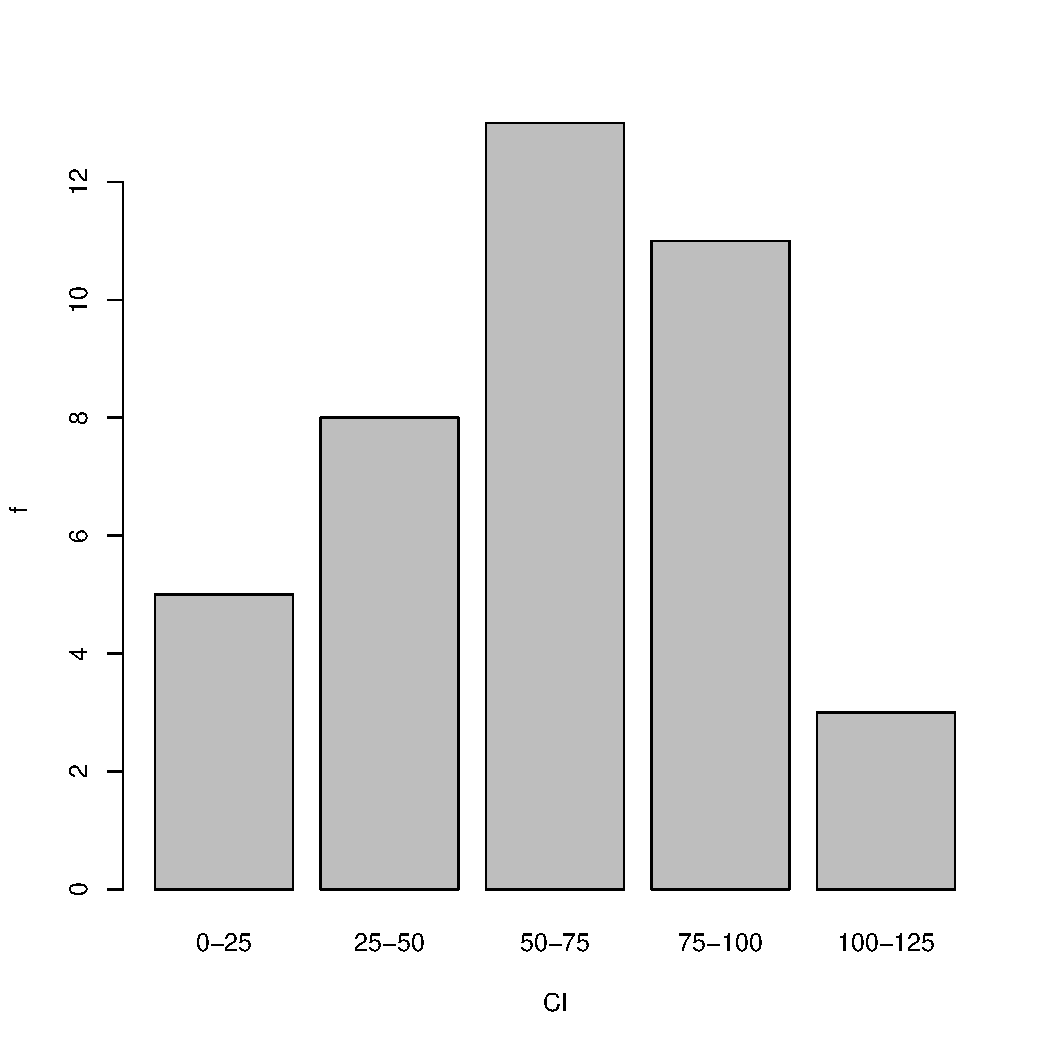
\includegraphics[width=\linewidth]{figures/end-term-paper/q5}
%------------------------------------------------------------------------------------------------------------------%
\end{document}